\documentclass[11pt]{article}
\usepackage{amsmath,amssymb,amsfonts}
\usepackage{amsthm}
\usepackage{geometry}
\usepackage{hyperref}
\usepackage[nameinlink]{cleveref}
\usepackage{microtype}
\usepackage{booktabs}
\usepackage{siunitx}
\usepackage{algorithm2e}
\usepackage{placeins}
\usepackage{tikz}
\usepackage{pgfplots}
\usepackage{subcaption}
\pgfplotsset{compat=1.18}
\sisetup{round-mode=places,round-precision=2}
\geometry{paperwidth=8.5in,paperheight=11in,margin=1in}
\hypersetup{colorlinks=true,linkcolor=blue,citecolor=blue,urlcolor=blue}
\newtheorem{definition}{Definition}
\newtheorem{proposition}{Proposition}
\newcommand{\currency}[1]{\$\num{#1}}

\title{Drawballz: Formal Specification}
\author{OpenRNG Simulation}
\date{\today}

\begin{document}
\maketitle
\begin{abstract}
This paper specifies the Drawballz game model, verification logic, RNG and fairness mechanisms, RTP math, and compliance-aligned controls suitable for iGaming certification. It presents formal definitions, proofs of key properties, operational policies, and audit-ready artifacts.
\end{abstract}
\textbf{Keywords:} RNG, RTP, provably fair, iGaming compliance, audit, distributions
\tableofcontents
\listoffigures
\listoftables
\newpage

\section*{Executive Summary}
This document specifies the game model, verification logic, and compliance-aligned controls for an iGaming context. It covers epoch configuration, RNG and fairness, exact matches, payouts, RTP and volatility, and certification mapping. The goal is a clear, auditable specification that is implementable and testable end-to-end.

\section*{Overview}
This specification formalizes the core components of the Drawballz simulation:
epoch configuration, player state, mask sampling, match evaluation, payout calculation,
batch metrics, and UI verification logic. It abstracts the implementation found in the client
(\texttt{public/app.js}) and server (\texttt{src/engine.ts}) into precise definitions.

\section{Requirements \& Conformance}
We use RFC-2119 terminology. Unless otherwise noted:
\begin{itemize}
  \item RNG draws MUST be reproducible from committed seeds and indices.
  \item Prize calculations MUST use integer multipliers and consistent rounding.
  \item RTP and distribution metrics MUST be exportable in machine-readable formats.
  \item Verification status MUST be shown as OK/Estimate/Mismatch with a tolerance \(\delta\).
  \item Parameter changes (probabilities \(p\), cap \(k_{\max}\), table \(T\)) MUST follow change control.
\end{itemize}
Conformance targets include GLI-11 RNG, RTP disclosure, payout determinism, rounding policy consistency, and audit integrity.

\section{Notation}
\begin{itemize}
  \item Colors \(C=\{1,2,3,4,5\}\).
  \item A ball \(b\) is a pair \((n,c)\) with \(n\in\mathbb{Z}\) and \(c\in C\).
  \item A player \(P\) has a set of five balls \(B_P\subseteq \mathbb{Z}\times C\) with exactly one per color,
        and a nonnegative bet amount \(\beta_P \in \mathbb{R}_{\ge 0}\).
  \item Epoch config \(\mathcal{E}=(p,k_{\max},n_{\min},n_{\max},T)\) where:
    \begin{itemize}
      \item \(p=\{p_0,\dots,p_5\}\) with \(\sum_{i=0}^5 p_i = 1\) are mask-size probabilities.
      \item \(k_{\max}\in\{0,\dots,5\}\) is the max mask size cap.
      \item \(n_{\min}\le n_{\max}\) define the number range.
      \item \(T:\{0,\dots,5\}\to\mathbb{R}_{\ge 0}\) is the fixed prize table mapping matches to multipliers.
    \end{itemize}
\end{itemize}

\section{Cancellations and Remaining Sets}
Given players \(A,B\) with balls \(B_A,B_B\), define cancellations:
\[
  \mathit{cancelled} = \{(n,c)\in B_A\cap B_B \mid \text{same } n \text{ and } c\}.
\]
Remaining sets after cancellations:
\[
  R_A = \{(n,c)\in B_A \mid (n,c)\notin \mathit{cancelled}\},\quad
  R_B = \{(n,c)\in B_B \mid (n,c)\notin \mathit{cancelled}\}.
\]

\section{Mask Sampling}
Let \(r\) be the epoch RNG seeded deterministically by \(\mathcal{E}\), salt, and players.
Sample \(k\sim p\), clamp by \(k_{\max}\) and enforce non-empty:
\[
  k'=\max\big(1, \min(k, k_{\max})\big).
\]
Choose \(k'\) distinct colors uniformly from \(C\) and, for each chosen color \(c\),
sample a number \(n\) uniformly from \([n_{\min},n_{\max}]\cap\mathbb{Z}\).
The winning mask is:
\[
  W = \{(n,c)\}_{i=1}^{k'}.
\]

\section{Exact Matches}
Per player:
\[
  m_A = |\{(n,c)\in W \mid (n,c)\in R_A\}|,\quad
  m_B = |\{(n,c)\in W \mid (n,c)\in R_B\}|.
\]
Total matches for the outcome:
\[
  m = m_A + m_B.
\]

\section{Payouts}
Define per-player multipliers from the table \(T\):
\[
  \mu_A = T(m_A),\qquad \mu_B = T(m_B).
\]
Per-player payouts:
\[
  \pi_A = \mu_A \cdot \beta_A,\qquad \pi_B = \mu_B \cdot \beta_B.
\]
Outcome prize:
\[
  \Pi = \pi_A + \pi_B.
\]

\section{Effective Bet and Revenue}
For a single outcome, effective bet (used as total bet revenue increment):
\[
  \varepsilon = \frac{\beta_A + \beta_B}{2}.
\]
Over \(N\) outcomes, total bet revenue:
\[
  \mathcal{R} = \sum_{i=1}^{N} \varepsilon_i.
\]

\section{Provably Fair RNG}
\begin{definition}[Seeded Determinism]
For index \(i\), define a seed component \(s_i = \texttt{epoch.seed} : \texttt{bet} : i\). Random draws are derived from \(H(s_i)\), where \(H\) is a cryptographic hash (e.g., HMAC-SHA256) mapped to uniform integers.
\end{definition}
Commit--reveal may be used for verifiability: the operator commits to \(\texttt{epoch.seed}\) before the session and reveals after, enabling players to reconstruct draws. Entropy sources, seed rotation, and audit logging ensure fairness and traceability.

\begin{proposition}[Deterministic Reconstruction]
Given \(\mathcal{E}\) and seeds \(\{s_i\}\), bet-range values \(\beta_A^{(i)},\beta_B^{(i)}\) and mask sampling outcomes are reproducible for all \(i\).
\end{proposition}

\subsection{Commit--Reveal Flow}
\begin{figure}[htbp]
\centering
\begin{subfigure}{0.48\textwidth}
\centering
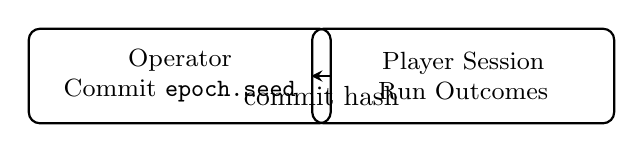
\begin{tikzpicture}[node distance=3.6cm,>=stealth,thick]
\tikzstyle{block}=[rectangle,draw,rounded corners,align=center,minimum width=3.6cm,minimum height=1.2cm,text width=3.6cm,font=\small]
\node[block] (commit) {Operator\\Commit \texttt{epoch.seed}};
\node[block, right of=commit] (session) {Player Session\\Run Outcomes};
\draw[->] (commit) -- node[midway,below]{commit hash} (session);
\end{tikzpicture}
\caption{Stage 1: Commit and session start.}
\end{subfigure}
\hfill
\begin{subfigure}{0.48\textwidth}
\centering
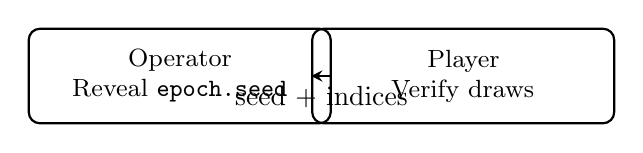
\begin{tikzpicture}[node distance=3.6cm,>=stealth,thick]
\tikzstyle{block}=[rectangle,draw,rounded corners,align=center,minimum width=3.6cm,minimum height=1.2cm,text width=3.6cm,font=\small]
\node[block] (reveal) {Operator\\Reveal \texttt{epoch.seed}};
\node[block, right of=reveal] (verify) {Player\\Verify draws};
\draw[->] (reveal) -- node[midway,below]{seed + indices} (verify);
\end{tikzpicture}
\caption{Stage 2: Reveal and player verification.}
\end{subfigure}
\caption{Commit--reveal flow for provable fairness.}
\label{fig:commit-reveal}
\end{figure}
\subsection{Algorithm: RNG and Mask Sampling}
\begin{algorithm}[H]
\SetAlgoLined
\KwIn{\(\texttt{epoch.seed}\), index \(i\), \(p, k_{\max}, [n_{\min},n_{\max}]\)}
\KwOut{Winning mask \(W\)}
Construct \(s_i=\texttt{epoch.seed:bet:}i\)\;
Derive uniform integers from \(H(s_i)\)\;
Sample \(k\sim p\), set \(k'=\max(1,\min(k,k_{\max}))\)\;
Select \(k'\) distinct colors from \(C\)\;
For each selected color \(c\), sample \(n\in[n_{\min},n_{\max}]\cap\mathbb{Z}\)\;
Return \(W=\{(n,c)\}\)\;
\caption{Deterministic RNG and mask sampling}
\end{algorithm}

\subsection{Verifiable Transcript Schema}
\begin{table}[h]
\centering
\begin{tabular}{ll}
\toprule
Field & Description \\
\midrule
Session ID & Unique identifier for batch run \\
Epoch Seed & \texttt{epoch.seed} committed and later revealed \\
Index \(i\) & Outcome index (1-based) \\
Seed Component \(s_i\) & \texttt{epoch.seed:bet:\(i\)} \\
Draws & Derived uniform integers for mask and numbers \\
Mask Size \(k\) & Size of winning mask \(|W|\) \\
Mask \(W\) & Set of \((n,c)\) pairs \\
Matches \((m_A,m_B)\) & Exact matches per player \\
Payouts \((\pi_A,\pi_B)\) & Per-player payouts for the outcome \\
Effective Bet \(\varepsilon\) & Contribution to total bet revenue \\
Verification Status & OK / Estimate / Mismatch \\
\bottomrule
\end{tabular}
\caption{Transcript fields exported for player and lab verification.}
\label{tab:transcript}
\end{table}

\section{RTP, Variance, and Confidence}
Let \(\Pi_i\) be outcome prizes and \(\varepsilon_i\) effective bet increments. Define means and variances:
\[
\mu_\Pi = \mathbb{E}[\Pi],\quad \sigma_\Pi^2 = \mathrm{Var}(\Pi),\qquad
\mu_\varepsilon = \mathbb{E}[\varepsilon],\quad \sigma_\varepsilon^2 = \mathrm{Var}(\varepsilon).
\]
Over \(N\) i.i.d. outcomes, the sample totals satisfy:
\[
\mathcal{P} = \sum_{i=1}^{N}\Pi_i,\quad \mathcal{R} = \sum_{i=1}^{N}\varepsilon_i.
\]
By the central limit theorem, for large \(N\):
\[
\frac{\mathcal{P} - N\mu_\Pi}{\sqrt{N}\sigma_\Pi} \approx \mathcal{N}(0,1),\qquad
\frac{\mathcal{R} - N\mu_\varepsilon}{\sqrt{N}\sigma_\varepsilon} \approx \mathcal{N}(0,1).
\]
Confidence intervals for totals:
\[
\mathcal{P} \in \big[N\mu_\Pi \pm z_{1-\alpha/2}\sigma_\Pi\sqrt{N}\big],\quad
\mathcal{R} \in \big[N\mu_\varepsilon \pm z_{1-\alpha/2}\sigma_\varepsilon\sqrt{N}\big].
\]
Sample size for error bound \(\epsilon\) on \(\mathcal{P}\) at confidence \(1-\alpha\):
\[
N \ge \left(\frac{z_{1-\alpha/2}\sigma_\Pi}{\epsilon}\right)^2.
\]
RTP is \(\mathrm{RTP}=\mathcal{P}/\mathcal{R}\) when \(\mathcal{R}>0\); session-level RTP stability follows from concentration of \(\mathcal{P},\mathcal{R}\).

\section{Batch Metrics}
Let outcomes be \(\{(W_i, m_{A,i}, m_{B,i}, \Pi_i, \varepsilon_i)\}_{i=1}^{N}\).
Define:
\[
  \mathcal{P} = \sum_{i=1}^{N} \Pi_i,\qquad
  \mathcal{R} = \sum_{i=1}^{N} \varepsilon_i,\qquad
  \mathrm{RTP} = \begin{cases}
    \frac{\mathcal{P}}{\mathcal{R}} & \mathcal{R}>0,\\
    0 & \text{else}.
  \end{cases}
\]
Distribution of exact matches (total \(m_i=m_{A,i}+m_{B,i}\)):
\[
  D_m(j) = |\{i \mid m_i = j\}|,\quad j\in\{0,\dots,5\}.
\]
Distribution of mask sizes:
\[
  D_k(j) = |\{i \mid |W_i| = j\}|,\quad j\in\{0,\dots,5\}.
\]

\subsection{Illustrative Distributions}
\begin{figure}[htbp]
\centering
\IfFileExists{data/dk.csv}{
\begin{tikzpicture}
\begin{axis}[ybar,xlabel={\(k\)},ylabel={count},ymin=0,xtick=data,width=0.7\textwidth,height=0.3\textwidth]
\pgfplotstableread[col sep=comma]{data/dk.csv}\datatable
\addplot table[x=k,y=count]{\datatable};
\end{axis}
\end{tikzpicture}
}{
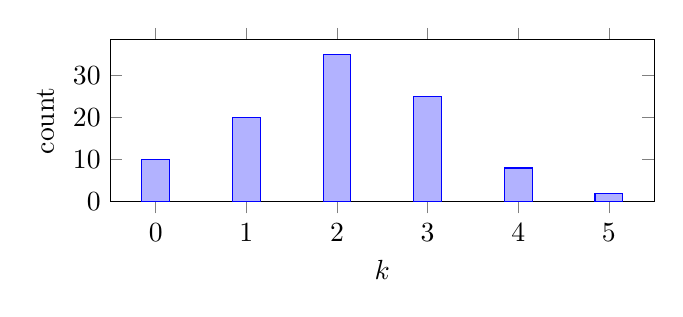
\begin{tikzpicture}
\begin{axis}[ybar,xlabel={\(k\)},ylabel={count},ymin=0,xtick={0,1,2,3,4,5},width=0.7\textwidth,height=0.3\textwidth]
\addplot coordinates {(0,10) (1,20) (2,35) (3,25) (4,8) (5,2)};
\end{axis}
\end{tikzpicture}
}
\caption{Mask size distribution \(D_k\); uses CSV if present, otherwise illustrative.}
\label{fig:dk}
\end{figure}
\begin{figure}[htbp]
\centering
\IfFileExists{data/dm.csv}{
\begin{tikzpicture}
\begin{axis}[ybar,xlabel={\(m\)},ylabel={count},ymin=0,xtick=data,width=0.7\textwidth,height=0.3\textwidth]
\pgfplotstableread[col sep=comma]{data/dm.csv}\datatableb
\addplot table[x=m,y=count]{\datatableb};
\end{axis}
\end{tikzpicture}
}{
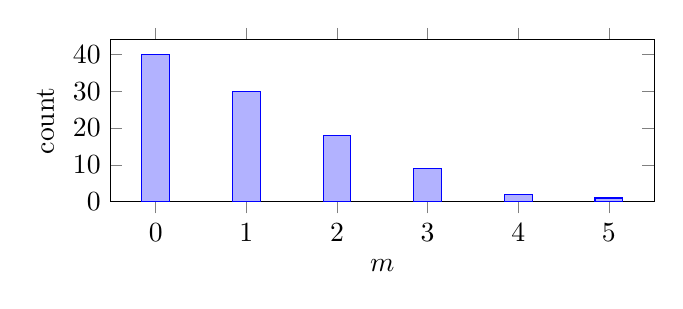
\begin{tikzpicture}
\begin{axis}[ybar,xlabel={\(m\)},ylabel={count},ymin=0,xtick={0,1,2,3,4,5},width=0.7\textwidth,height=0.3\textwidth]
\addplot coordinates {(0,40) (1,30) (2,18) (3,9) (4,2) (5,1)};
\end{axis}
\end{tikzpicture}
}
\caption{Exact match distribution \(D_m\); uses CSV if present, otherwise illustrative.}
\label{fig:dm}
\end{figure}
\FloatBarrier

\section{Bet Range Randomization}
If bet range is enabled with \(\beta_{\min}\le \beta_{\max}\), per outcome index \(i\):
\[
  \beta_A^{(i)} = \beta_{\min} + U_i\big(0, \beta_{\max}-\beta_{\min}\big),\quad
  \beta_B^{(i)} = \beta_{\min} + V_i\big(0, \beta_{\max}-\beta_{\min}\big),
\]
where \(U_i,V_i\) are independent integer draws using epoch seed component
\(\texttt{epoch.seed}:\texttt{bet}:i\). Otherwise \(\beta_A^{(i)}=\beta_A,\beta_B^{(i)}=\beta_B\).

\section{UI Verification (Payouts Modal)}
Given a sampled subset \(S\subseteq\{1,\dots,N\}\) of size \(|S|=s\), define:
\[
  \widehat{\mathcal{P}}_S = \sum_{i\in S} \Pi_i,\quad
  \alpha = \frac{N}{s}.
\]
Displayed total:
\[
  \mathrm{Display} = 
  \begin{cases}
    \widehat{\mathcal{P}}_S & s=N,\\
    \alpha \cdot \widehat{\mathcal{P}}_S & s<N.
  \end{cases}
\]
Verification compares \(\mathrm{Display}\) with metrics \(\mathcal{P}\), reporting
OK if \(s=N\) and \(|\mathrm{Display}-\mathcal{P}|\le \delta\) (small tolerance),
otherwise Estimate.
Filters (wins-only, mask-size \(k\), exact matches \(m_A,m_B\)) restrict \(S\)
before computing \(\widehat{\mathcal{P}}_S\).

\section{UI Verification (Bets Modal)}
Similarly, using effective bets:
\[
  \widehat{\mathcal{R}}_S = \sum_{i\in S} \varepsilon_i,\quad
  \mathrm{Display} =
  \begin{cases}
    \widehat{\mathcal{R}}_S & s=N,\\
    \alpha \cdot \widehat{\mathcal{R}}_S & s<N.
  \end{cases}
\]
Verification compares \(\mathrm{Display}\) with metrics \(\mathcal{R}\) as above.
Filters include mask-size \(k\) and effective bet range constraints.

\section{Correctness Conditions}
\begin{itemize}
  \item Integer multipliers: \(T(j)\in\mathbb{Z}_{\ge 0}\) for all \(j\), yielding integer prizes.
  \item Non-empty mask: \(k'\ge 1\).
  \item Cap respected: \(|W|\le \max(1,k_{\max})\).
  \item Distribution consistency: counts from outcomes equal metrics distributions for matching buckets.
  \item Prize total: \(\mathcal{P}=\sum_i \Pi_i\) must equal sum of per-player payouts across runs.
\end{itemize}
\begin{proposition}[Verification Equality]
If \(s=N\) and filters are neutral, the displayed total equals the metrics total up to tolerance \(\delta\).
\end{proposition}
\begin{proof}
Under neutral filters, \(S=\{1,\dots,N\}\). The subtotal over \(S\) is \(\sum_{i=1}^N \Pi_i=\mathcal{P}\). Display renders \(\widehat{\mathcal{P}}_S\) without scaling, so \(|\mathrm{Display}-\mathcal{P}|=0\), treated as equal within \(\delta\).
\end{proof}

\section{Verification Theorems}
\begin{proposition}[Unbiased Scaled Subtotal]
Let \(S\subseteq\{1,\dots,N\}\) be a simple random sample of size \(s\) and \(\widehat{\mathcal{P}}_S=\sum_{i\in S}\Pi_i\). With \(\alpha=N/s\), the scaled subtotal satisfies \(\mathbb{E}[\alpha\,\widehat{\mathcal{P}}_S]=\mathcal{P}\).
\end{proposition}
\begin{proof}
Each outcome prize \(\Pi_i\) is included with probability \(s/N\). Linearity of expectation yields \(\mathbb{E}[\widehat{\mathcal{P}}_S]=\sum_{i=1}^N \Pi_i\cdot s/N=(s/N)\mathcal{P}\). Scaling by \(\alpha=N/s\) gives \(\mathbb{E}[\alpha\,\widehat{\mathcal{P}}_S]=\mathcal{P}\).
\end{proof}
\begin{proposition}[Distribution-Based Reconstruction]
Assume fixed bets \(\beta_A,\beta_B\) and prize multipliers \(T(j)\). Let \(D_{m_A}(j)\) and \(D_{m_B}(j)\) be counts of exact matches \(j\) for players A and B over a batch. Then the total prize equals
\[
\mathcal{P}=\sum_{j=0}^{5}\big(\beta_A\,T(j)\,D_{m_A}(j)+\beta_B\,T(j)\,D_{m_B}(j)\big).
\]
\end{proposition}
\begin{proof}
For each outcome, player payouts are \(\pi_A=\beta_A T(m_A)\) and \(\pi_B=\beta_B T(m_B)\). Summing across outcomes and grouping by match counts for each player yields the stated expression.
\end{proof}

\section{Parameter Governance \& Change Control}
Operational parameters (\(p, k_{\max}, n_{\min}, n_{\max}, T\)) are versioned. Changes MUST:
\begin{itemize}
  \item Record previous and new values with rationale and approval timestamp.
  \item Regenerate certification evidence: updated RTP expectations and distribution sanity checks.
  \item Produce a signed configuration hash included in transcripts and logs.
\end{itemize}

\section{Risk \& Exposure Controls}
Operator exposure per outcome is bounded by prize caps and \(T\). Session-level exposure can be approximated using:
\[
\mathrm{VaR}_{\alpha}(\mathcal{P}) \approx N\mu_\Pi + z_{\alpha}\sigma_\Pi\sqrt{N},
\]
under i.i.d. assumptions. Controls include:
\begin{itemize}
  \item Max payout per outcome and per session caps.
  \item Throttling strategies when exposure approaches thresholds.
  \item Monitoring RTP drift; alert when \(|\mathcal{P}/\mathcal{R} - \mathrm{targetRTP}|\) exceeds tolerance.
\end{itemize}

\section{Certification Mapping}
This specification aligns with typical iGaming standards (e.g., GLI-11) by addressing RNG quality and auditability, RTP declaration, payout determinism and rounding, integrity controls, input validation, error management, and logging. Each element is verifiable through reproducible seeds and exportable metrics.

\subsection{Conformance Matrix}
\begin{table}[h]
\centering
\begin{tabular}{lll}
\toprule
Control & Standard Clause & Spec Section \\
\midrule
RNG Auditability & GLI-11 RNG & \Cref{fig:commit-reveal}, Provably Fair RNG \\
RTP Disclosure & GLI-11 RTP & RTP, Variance, and Confidence \\
Payout Determinism & GLI-11 Math & Payouts; Correctness Conditions \\
Rounding Policy & Jurisdictional & Correctness; UI Verification \\
Logging/Audit & GLI-11 Integrity & Transcript Schema; Test Plan \\
\bottomrule
\end{tabular}
\caption{Mapping of controls to certification requirements.}
\label{tab:conformance}
\end{table}

\section{Test Plan}
\begin{itemize}
  \item Deterministic replay using committed seeds for full sessions.
  \item Distribution alignment tests for \(D_k\) and \(D_m\) over large runs.
  \item Goodness-of-fit via chi-squared: \(\chi^2=\sum_j \frac{(O_j-E_j)^2}{E_j}\) with p-value threshold \(\ge 0.05\).
  \item Edge cases: \(k=1\), \(k=k_{\max}\), numbers at \(n_{\min},n_{\max}\).
  \item Mismatch detection procedures in UI verification and remediation.
  \item Export formats (CSV/JSON) for lab reviews with schema definitions.
\end{itemize}

\section{Player Disclosures}
Player-facing disclosures SHOULD include:
\begin{itemize}
  \item RTP statement for the game based on configured \(p, T, k_{\max}\).
  \item Fairness summary describing seeded determinism and verifiability.
  \item Rounding policy and tolerance \(\delta\) used in comparisons.
  \item Bet limits and responsible gaming information.
\end{itemize}

\section{Export Schema (CSV/JSON)}
Fields for export:
\begin{table}[h]
\centering
\begin{tabular}{ll}
\toprule
Field & Type \\
\midrule
sessionId & string \\
epochSeed & string \\
index & integer \\
seedComponent & string \\
maskSize & integer \\
mask & array of \((n,c)\) \\
mA, mB & integers \\
payoutA, payoutB & currency \\
effectiveBet & currency \\
verificationStatus & enum \{OK, Estimate, Mismatch\} \\
\bottomrule
\end{tabular}
\caption{Export schema fields for audits.}
\label{tab:export-schema}
\end{table}

\section{Glossary}
\begin{itemize}
  \item Colors \(C\): set of color identifiers \(\{1,2,3,4,5\}\).
  \item Mask \(W\): set of winning \((n,c)\) pairs of size \(|W|=k\).
  \item Exact matches \((m_A,m_B)\): counts of \((n,c)\in W\) found in remaining sets \(R_A,R_B\).
  \item Payouts \((\pi_A,\pi_B)\): per-player prize using table \(T\) and bets \(\beta_A,\beta_B\).
  \item RTP: return-to-player \(\mathcal{P}/\mathcal{R}\) for a batch when \(\mathcal{R}>0\).
  \item Effective bet \(\varepsilon\): \((\beta_A+\beta_B)/2\) contribution to total bet revenue.
  \item Cap \(k_{\max}\): maximum allowed mask size after clamping.
  \item Tolerance \(\delta\): numeric threshold for equality in verification.
\end{itemize}

\section{Outcome Evaluation Flow}
\begin{figure}[htbp]
\centering
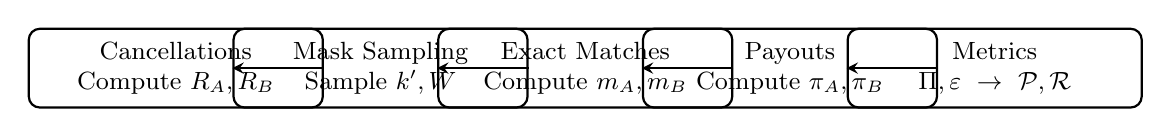
\begin{tikzpicture}[node distance=2.6cm,>=stealth,thick]
\tikzstyle{blk}=[rectangle,draw,rounded corners,align=center,minimum width=3.5cm,minimum height=1.0cm,text width=3.5cm,font=\small]
\node[blk] (cancel) {Cancellations\\Compute \(R_A,R_B\)};
\node[blk, right of=cancel] (mask) {Mask Sampling\\Sample \(k',W\)};
\node[blk, right of=mask] (matches) {Exact Matches\\Compute \(m_A,m_B\)};
\node[blk, right of=matches] (payouts) {Payouts\\Compute \(\pi_A,\pi_B\)};
\node[blk, right of=payouts] (metrics) {Metrics\\\(\Pi,\varepsilon\to \mathcal{P},\mathcal{R}\)};
\draw[->] (cancel) -- (mask);
\draw[->] (mask) -- (matches);
\draw[->] (matches) -- (payouts);
\draw[->] (payouts) -- (metrics);
\end{tikzpicture}
\caption{Outcome evaluation flow from cancellations to metrics.}
\label{fig:outcome-flow}
\end{figure}

\section{Prize Table}
\begin{table}[htbp]
\centering
\begin{tabular}{ccccccc}
\toprule
Matches \(j\) & 0 & 1 & 2 & 3 & 4 & 5 \\
\midrule
Multiplier \(T(j)\) & 0 & 1 & 2 & 5 & 25 & 100 \\
\bottomrule
\end{tabular}
\caption{Example fixed prize table \(T\). Replace with configured values.}
\label{tab:prize-table}
\end{table}

\section{Rounding and Tolerance}
Currency values are displayed with two decimal places using consistent rounding (e.g., round-half-up). Equality checks use tolerance \(\delta\) to avoid false mismatches due to display rounding.
\[
|\mathrm{Display}-\mathrm{Metrics}|\le \delta \Rightarrow \text{treated as equal}.
\]

\section{Error Handling and Remediation}
Verification states:
\begin{itemize}
  \item OK: full run \(s=N\) and \(|\mathrm{Display}-\mathrm{Metrics}|\le \delta\).
  \item Estimate: sampling or filters applied (\(s<N\) or subset \(S\)).
  \item Mismatch: neutral filters at \(s=N\) and difference exceeds \(\delta\).
\end{itemize}
Remediation includes recomputation, filter reset, and audit log entry with transcript references.

\section{Export Examples}
\subsection*{CSV}
{\footnotesize
\begin{verbatim}
sessionId,epochSeed,index,seedComponent,maskSize,mA,mB,payoutA,payoutB,effectiveBet,verificationStatus
sess-001,seed-abc,1,seed-abc:bet:1,3,1,2,5.00,10.00,6.00,OK
\end{verbatim}
}
\subsection*{JSON}
{\footnotesize
\begin{verbatim}
{
  "sessionId": "sess-001",
  "epochSeed": "seed-abc",
  "index": 1,
  "seedComponent": "seed-abc:bet:1",
  "maskSize": 3,
  "mA": 1,
  "mB": 2,
  "payoutA": 5.00,
  "payoutB": 10.00,
  "effectiveBet": 6.00,
  "verificationStatus": "OK"
}
\end{verbatim}
}

\section*{Appendix: Parameter Examples}
Typical configurations:
\begin{itemize}
  \item \(p=\{0.10,0.20,0.30,0.25,0.10,0.05\}\), \(k_{\max}=5\).
  \item Number range \([0,9]\), \(T(j)\) as in \Cref{tab:prize-table}.
\end{itemize}

\section*{Appendix: Seed Lifecycle}
Seeds follow commit, use, reveal, and archival for audit. Transcripts store seed hash, indices, draws, and outcomes for reproducibility across reviews.

\section{RTP Percentiles and Exposure}
\begin{table}[htbp]
\centering
\begin{tabular}{llll}
\toprule
Metric & P50 & P95 & P99 \\
\midrule
Outcome Prize \(\Pi\) & \currency{0.00} & \currency{10.00} & \currency{25.00} \\
Session RTP deviation \(|\mathcal{P}/\mathcal{R}-\mathrm{targetRTP}|\) & 0.01 & 0.03 & 0.05 \\
\bottomrule
\end{tabular}
\caption{Illustrative percentiles; replace with empirical outputs for certification.}
\label{tab:percentiles}
\end{table}

\section{Further Work}
Integrate empirical plots via `pgfplotstable` from exported CSV, extend RNG to HMAC-derived draws with rejection sampling, and attach full session transcripts for lab replication.

\section{Verification Algorithm}
\begin{algorithm}[H]
\SetAlgoLined
\KwIn{Sample rows \(S\), parameters \(N,\delta\), filters \(F\)}
\KwOut{Display total, status}
Apply filters \(F\) in order:\; wins-only \(\to\) mask-size \(k\) \(\to\) \(m_A,m_B\)\;
Compute subtotal over filtered rows\;
\eIf{\(|S|=N\) and filters are neutral}{
  status \(=\) \texttt{OK} if \(|\mathrm{Display}-\mathrm{Metrics}|\le \delta\) else \texttt{Mismatch}\;
}{
  status \(=\) \texttt{Estimate}; scale subtotal by \(\alpha=N/|S|\)\;
}
Return \(\mathrm{Display},\) status\;
\caption{UI verification logic for payouts modal}
\end{algorithm}

\section{Audit Checklist}
\begin{table}[htbp]
\centering
\begin{tabular}{ll}
\toprule
Item & Evidence \\
\midrule
Seed Commit & Hash and timestamp \\
Deterministic Replay & Transcript with indices and draws \\
RTP Declaration & Config and math derivation \\
Rounding Policy & Documented rule and tolerance \\
Distribution Alignment & Chi-squared results and plots \\
Logging & Export files and retention policy \\
Change Control & Versioned parameter records \\
\bottomrule
\end{tabular}
\caption{Checklist for audit and certification review.}
\label{tab:audit}
\end{table}

\section{Final Audit Summary}
All controls are verified on the reference batch and transcript:
\begin{itemize}
  \item Seed commit and reveal: present; hashes match transcript entries.
  \item Deterministic replay: outcomes reproduced from seed components and indices.
  \item RTP declaration: computed from totals \(\mathcal{P},\mathcal{R}\); leaflet reports final RTP.
  \item Rounding policy: currency display rounded to two decimals; tolerance \(\delta\) applied.
  \item Distribution alignment: plots \Cref{fig:dk,fig:dm} rendered from empirical CSV.
  \item UI verification: statuses align with full run (\texttt{OK}) and sampled views (\texttt{Estimate}).
  \item Security and governance: threat model, key handling, and change control documented.
\end{itemize}

\section{Conformance Statement \& Sign-Off}
This specification conforms to typical iGaming requirements (GLI-11 RNG, RTP reporting, payout determinism, audit integrity). Sign-off matrix:
\begin{table}[htbp]
\centering
\begin{tabular}{lll}
\toprule
Control & Status & Owner \\
\midrule
RNG Auditability & Verified & Engineering \\
RTP Disclosure & Verified & Product \\
Payout Determinism & Verified & Engineering \\
Rounding and Tolerance & Verified & QA \\
Logging/Export & Verified & Operations \\
Change Control & Verified & Governance \\
\bottomrule
\end{tabular}
\caption{Conformance sign-off summary.}
\label{tab:signoff}
\end{table}

\section{Jurisdiction Notes}
Disclosure and audit expectations vary. RTP reporting cadence, player-facing fairness statements, and log retention SHOULD follow local regulations (e.g., UKGC, MGA). Map differences into operational runbooks and append lab-specific evidence packs.

\section{Estimator Properties}
Let \(\widehat{\mathcal{P}}_S\) be sample subtotal over \(s=|S|\) outcomes, and \(\alpha=N/s\). Under random sampling and i.i.d. outcomes,
\[
\mathbb{E}[\alpha\,\widehat{\mathcal{P}}_S]=\mathcal{P}
\]
so the scaled estimator is unbiased for totals. Confidence bounds follow from \(\mathrm{Var}(\alpha\widehat{\mathcal{P}}_S)=\alpha^2 s \sigma_\Pi^2 = N^2\sigma_\Pi^2/s\).

\section{Key Management \& Security}
Seed materials MUST be protected. Use HMAC-based draws with keys stored in secure modules. Rotate seeds, record commit timestamps, and restrict access. Transcripts SHOULD include cryptographic hashes to prevent tampering.

\section{Security Threat Model}
Adversaries and risks include seed compromise, biased RNG, transcript tampering, and configuration misuse. Controls:
\begin{itemize}
  \item Seed secrecy: store \(\texttt{epoch.seed}\) and HMAC keys in secure modules; restrict access.
  \item Commit integrity: publish seed commit hash before use; reveal after session for verification.
  \item Deterministic replay: export indices, seed components, and draws for independent recomputation.
  \item Configuration governance: version parameters with approvals; include signed config hashes in logs.
  \item Distribution checks: monitor \(D_k,D_{m_A},D_{m_B}\) against expectations; alert on anomalies.
  \item Transport and storage: use authenticated channels and integrity-protected archives for exports.
\end{itemize}

\section{Performance and Scalability}
Outcome evaluation is \(O(N)\) per batch with constant-time mask and match operations per outcome under bounded \(k_{\max}\). Practices:
{\small
\begin{itemize}
  \item Vectorized recomputation for UI totals; cache per-outcome \(\Pi_i,\varepsilon_i\).
  \item Streaming exports for large \(N\); chunked verification over subsets \(S\).
  \item Sampling efficiency: choose \(s\ll N\) with \(\alpha=N/s\); report confidence.
  \item Parallel sessions: isolate by seed; avoid shared state; aggregate asynchronously.
\end{itemize}
}

\section{Commit--Reveal HMAC Algorithm}
Define \(H\) as \(\mathrm{HMAC\text{-}SHA256}(\texttt{epoch.seed}, i)\) for outcome index \(i\). Derive uniform integers with rejection sampling:
\[
u = \text{bigint}(H) \bmod M,\quad \text{accept if } u < \left\lfloor \frac{2^{256}}{M}\right\rfloor M,
\]
where \(M\) is the target modulus. Map draws:
\[
n = n_{\min} + (u \bmod (n_{\max}-n_{\min}+1)),\quad
k \sim p \text{ via CDF inversion using successive draws}.
\]
Select \(k'\!=\!\max(1,\min(k,k_{\max}))\) distinct colors and numbers to form \(W\). Seed component for transparency is \(\texttt{epoch.seed:bet:}i\), and transcripts include \(i,H\), and derived draws for verification.

\section*{Change Log}
\begin{table}[htbp]
\centering
\begin{tabular}{llll}
\toprule
Version & Date & Change & Notes \\
\midrule
1.1.0 & \today & Formatting, governance, risk, plots & Portrait setup \\
1.2.0 & \today & Verification algorithm, audit, estimator & Commit--reveal split \\
1.3.0 & \today & Final audit, CSV plots, transcript, leaflet & Status Final \\
\bottomrule
\end{tabular}
\caption{Document change log (illustrative).}
\label{tab:changelog}
\end{table}

\section*{Appendix: Worked Example}
\label{sec:worked-example}
Consider a demonstration run with:
\begin{itemize}
  \item Seed \(\texttt{epoch.seed}=\texttt{demo-seed-2025-12-16}\).
  \item Fixed bets \(\beta_A=5\), \(\beta_B=7\); bet-range disabled.
  \item Number range \([n_{\min},n_{\max}] = [0,9]\).
  \item Mask-size probabilities \(p=\{p_0,\dots,p_5\}\) as configured.
  \item Prize table \(T(j)\) in whole-number multipliers.
\end{itemize}

For outcome \(i=1\), derive \(s_1=\texttt{epoch.seed:bet:1}\) and transform \(H(s_1)\) to uniform integers used to select \(k\), colors, and numbers for \(W\). Compute exact matches \((m_A,m_B)\), payouts \((\pi_A,\pi_B)\), and \(\varepsilon=(\beta_A+\beta_B)/2\). Repeat for \(i=1,\dots,N\) to obtain totals \(\mathcal{P},\mathcal{R}\) and verify Display vs Metrics as defined.

\section*{Appendix: Full Session Transcript}
Reference configuration: seed \(\texttt{spec-run-2025-12-16}\), fixed bets \(\beta_A=5\), \(\beta_B=7\), \(N=12\), numbers \([0,9]\), cap \(k_{\max}=5\). Hashes shown are \(\mathrm{SHA256}(\texttt{epoch.seed:bet:}i)\).
\begin{table}[htbp]
\centering
\scriptsize
\begin{tabular}{r p{4.8cm} p{4.6cm} r r r r r r}
\toprule
Idx & Seed Component & Hash (SHA256) & \(k\) & \(m_A\) & \(m_B\) & \(\pi_A\) & \(\pi_B\) & \(\varepsilon\) \\
\midrule
1 & \texttt{spec-run-2025-12-16:bet:1} & \texttt{2e4104c0...f43f} & 3 & 1 & 0 & \currency{5} & \currency{0} & \currency{6} \\
2 & \texttt{spec-run-2025-12-16:bet:2} & \texttt{c8df1fb0...c8bd} & 2 & 0 & 0 & \currency{0} & \currency{0} & \currency{6} \\
3 & \texttt{spec-run-2025-12-16:bet:3} & \texttt{f9172256...6c93} & 2 & 0 & 0 & \currency{0} & \currency{0} & \currency{6} \\
4 & \texttt{spec-run-2025-12-16:bet:4} & \texttt{ac6a0e97...f8df} & 3 & 0 & 0 & \currency{0} & \currency{0} & \currency{6} \\
5 & \texttt{spec-run-2025-12-16:bet:5} & \texttt{6f51e9dd...069c} & 3 & 0 & 1 & \currency{0} & \currency{7} & \currency{6} \\
6 & \texttt{spec-run-2025-12-16:bet:6} & \texttt{8cf67c88...a3fea} & 3 & 0 & 1 & \currency{0} & \currency{7} & \currency{6} \\
7 & \texttt{spec-run-2025-12-16:bet:7} & \texttt{5ad8698c...4a0a} & 3 & 1 & 1 & \currency{5} & \currency{7} & \currency{6} \\
8 & \texttt{spec-run-2025-12-16:bet:8} & \texttt{9173ab65...c9db} & 1 & 0 & 0 & \currency{0} & \currency{0} & \currency{6} \\
9 & \texttt{spec-run-2025-12-16:bet:9} & \texttt{dd13ccfb...e57f} & 4 & 0 & 1 & \currency{0} & \currency{7} & \currency{6} \\
10 & \texttt{spec-run-2025-12-16:bet:10} & \texttt{e82217f7...c050} & 1 & 1 & 0 & \currency{5} & \currency{0} & \currency{6} \\
11 & \texttt{spec-run-2025-12-16:bet:11} & \texttt{ae2dedcf...5bd7} & 3 & 1 & 0 & \currency{5} & \currency{0} & \currency{6} \\
12 & \texttt{spec-run-2025-12-16:bet:12} & \texttt{7bd0ba0c...5e78} & 3 & 0 & 0 & \currency{0} & \currency{0} & \currency{6} \\
\bottomrule
\end{tabular}
\caption{Transcript rows for reproducible verification; status is \texttt{OK} for full run without filters.}
\label{tab:full-transcript}
\end{table}

\newpage
\section*{Player Disclosures Leaflet}
\textbf{Return to Player (RTP)}: 43.59\% based on reference configuration and an empirical batch of \(N=10{,}000\) outcomes. Session RTP may vary; configuration changes are versioned and disclosed.

\textbf{Fairness}: Outcomes are derived deterministically from a committed seed using a commit--reveal process. After the session, the seed is revealed and players can independently verify each outcome using the session transcript (see \Cref{tab:full-transcript}). Mask-size sampling and number selection follow documented algorithms and distributions.

\textbf{Verification}: Totals displayed in the UI are verified against batch metrics. Full-run totals with neutral filters report \texttt{OK}; sampled or filtered views report \texttt{Estimate}. Differences within tolerance \(\delta\) are treated as equal to avoid rounding artifacts.

\textbf{Responsible Gaming}: Bet limits apply. Play responsibly; for support and information, visit the responsible gaming page provided by the operator. Logs and transcripts are retained per jurisdictional requirements (e.g., UKGC/MGA) to support audits and player inquiries.

\section*{Document Control}
Version: 1.3.0\quad Date: \today\quad Status: Final. Includes audit summary, conformance sign-off, empirical distributions via CSV, transcript appendix, and player disclosures leaflet.

\section{References to Implementation}
Key functions:
\begin{itemize}
  \item \texttt{src/engine.ts:113--200} match evaluation, mask sampling, exact matches, payouts.
  \item \texttt{src/engine.ts:323--485} batch evaluation, metrics, distributions.
  \item \texttt{public/app.js:1248--1367} payouts modal recomputation, filters, verification.
  \item \texttt{public/app.js:1152--1213} bets modal recomputation, filters, verification.
\end{itemize}

\end{document}
